\documentclass[t,11pt]{beamer}

% Theme
\usetheme[faculty=sciences,lang=en,rmfont=pmn,logofont=fpi]{leiden}

% Packages
\usepackage{epstopdf}
\usepackage{tabularx}
\usepackage[compatibility=false]{caption}
\usepackage{subcaption}
\usepackage{mdframed}

% Timeline
\newcommand{\timeline}{\color{white}\makebox[0pt]{\textbullet}\hskip-0.5pt\vrule width 1pt\hspace{\labelsep}}

% Package configuration
\makeatletter
\@addtoreset{subfigure}{framenumber}% subfigure counter resets every frame
\makeatother
\DeclareGraphicsExtensions{.pdf,.eps,.png,.jpg}

% Template overrides
\mathversion{normal}
\usefonttheme{professionalfonts}

\setbeamerfont{title}{size=\Huge,series=}
\setbeamerfont{subtitle}{size=\small}
\setbeamerfont{frametitle}{series=}
\setbeamerfont{title in head/foot}{size=\scriptsize}
\setbeamerfont{author in head/foot}{size=\scriptsize}
\setbeamerfont{subtitle}{size=\footnotesize}

\setbeameroption{hide notes}
\setbeamertemplate{footline}{\fontsize{12}{25}\selectfont~\insertframenumber/\inserttotalframenumber}
\def\headlinepresentationtitle{%
\usebeamerfont{title in head/foot}%
\usebeamercolor[fg]{title in head/foot}%
  \leavevmode%
  \hbox{%
    \begin{beamercolorbox}[wd=.50\linewidth,ht=2.25ex,dp=1ex,left]{title in
      head/foot}%
      \insertlecture%
    \end{beamercolorbox}%
    \begin{beamercolorbox}[wd=.50\linewidth,ht=2.25ex,dp=1ex,right]{title in
      head/foot}%
      \insertauthor
    \end{beamercolorbox}%
  }
  \vskip0pt%
}
\nonstopmode

% Template configuration
\lecture[Leiden Template]{Distributed sentiment analysis on GitHub commit comments}{ldn-bmr}
\title{Distributed sentiment analysis on GitHub commit comments}
\subtitle{Seminar Distributed Data Mining}
\date{\now}
\author{Leon Helwerda, Tim van der Meij}

\begin{document}

% Opening slide
{\setbeamertemplate{navigation symbols}{}
\begin{frame}[plain]
  \maketitle
\end{frame}
\addtocounter{framenumber}{-1}}

\toggleslidecolors

% Regular slide
\setbeamertemplate{navigation symbols}{}
\begin{frame}[fragile]{Contents}
\begin{itemize}
  \item Introduction
  \item Problem statement
  \item Dataset
  \item Implementation
  \item Experiments and results
  \item Conclusion
\end{itemize}
\end{frame}

% Regular slide
\setbeamertemplate{navigation symbols}{}
\begin{frame}[fragile]{Introduction}
\begin{itemize}
  \item Sentiment analysis: extract subjective information (emotions)
  \item GitHub commit comments: review comments on code
  \item Not an easy task: natural language processing, large amounts of data
  \item Processing needs to be fast to be feasible
  \item Distribute most tasks onto worker nodes
\end{itemize}
\end{frame}

% Regular slide
\setbeamertemplate{navigation symbols}{}
\begin{frame}[fragile]{Problem statement}
\begin{itemize}
  \item Commit comment: (mostly) positive, negative or neutral?
  \item Initial idea: use positive and negative word lists
  \item Final idea: use a classifier with a training and test set
\end{itemize}
\begin{itemize}
  \item How do we obtain the dataset and preprocess it?
  \item How do we obtain labeled training data?
  \item What is the best classifier to use?
  \item How can we distribute the work onto worker nodes?
\end{itemize}
\end{frame}

% Regular slide
\setbeamertemplate{navigation symbols}{}
\begin{frame}[fragile]{Dataset}
\vspace*{-26pt}
\begin{table}[h]
  \centering
  {\setlength{\tabcolsep}{3pt}\footnotesize
  \begin{tabular}{|l|r|l|} \hline
    Dump                       &   \# items & Size \\ \hline
    2015-01-29 commit comments &    182.282 & 43~MB compressed, 267~MB BSON
    \\ \hline
    2015-01-29 Latin-only      &    165.427 & 42~MB processed JSON \\ \hline
    Commit comments (17 dumps) &  1.731.251 & 434~MB compressed \\ \hline
    Repositories (languages)   & 12.802.797 & 10.8~GB compressed, 1.3~GB shelf 
    \\ \hline
  \end{tabular}}
\end{table}
\begin{itemize}
  \item GHTorrent project: bimonthly dumps from GitHub API
  \item Commit comments, issue comments, events, repositories\ldots
  \item BSON $\to$ JSON $\to$ preprocessor, example entry:
\end{itemize}
{\scriptsize\begin{verbatim}
{
    "id": 8771097,
    "body": "It seems e.offsetX is not the way to get the relative
             cursor position in Firefox. I'm getting `undefined' in
             my experiments there.",
    "url": "https://api.github.com/repos/fedwiki/wiki-plugin-method/
            comments/8771097"
}
\end{verbatim}}
\end{frame}

% Regular slide
\setbeamertemplate{navigation symbols}{}
\begin{frame}[fragile]{Implementation}
{%
  \vspace{0.5cm}
  \setlength\extrarowheight{6pt}
  \begin{tabular}{@{\,}r <{\hskip 2pt}!{\timeline}
>{\raggedright\arraybackslash}p{9.5cm}}
    & Setting up environment on DAS-3, extensive README \\
    & Implementation of positive/negative word lists approach \\
    & Implementation of automatic dataset download/extraction \\
    & Addition of new words and smileys after data inspection \\
    & Better word splitting and non-Latin message filter \\
    & Implementation of labeler and colored output \\
    & First implementation of classifier with MapReduce support \\
    & Code refactoring: component framework, memory reduction \\
    & Manually labeling 2000 training examples \\
  \end{tabular}
}
\end{frame}

% Regular slide
\setbeamertemplate{navigation symbols}{}
\begin{frame}[fragile]{Implementation (continued)}
{%
  \vspace{0.5cm}
  \setlength\extrarowheight{6pt}
  \begin{tabular}{@{\,}r <{\hskip 2pt}!{\timeline} >{\raggedright\arraybackslash}p{9.5cm}}
    & Generic preprocessor: download, extract, convert and filter fields \\
    & Optimizations: more cores, shelves and extraction, model output \\
    & Plot script for various results and output/display formats \\
    & Implementation of repositories preprocessing \\
    & Distributed processing (MPI) for repository dumps \\
    & Research on classifiers/regressors and parameters, cross-validation \\
    & Implementation of experiment runner with plotter \\
    & Distributed processing (MPI) for commit comments dumps \\
  \end{tabular}
}
\end{frame}

% Regular slide
% TODO: passive aggressive is better than random forest, so why are the 
% language plots made with a random forest regressor? Determine which algorithm 
% to use for this.
\setbeamertemplate{navigation symbols}{}
\begin{frame}[fragile]{Experiments and results}
\begin{itemize}
  \item Determining best classifier to use
  \item Manifest with 15 different classifiers
  \item Using experiment runner to test various configurations
  \item Best scores on training set: linear SVC, passive aggressive and random 
    forest
  \item Complexity and interpretability of model varies
  \item Regressor variants score worse due to discrete class labels, but smooth 
    score curves may be benefit
\end{itemize}
\end{frame}

% Regular slide
\setbeamertemplate{navigation symbols}{}
\begin{frame}[fragile]{Experiments and results (continued)}
\vspace*{-26pt}
  \begin{figure}
    \centering
    \begin{subfigure}[b]{0.6\textwidth}
      \centering
      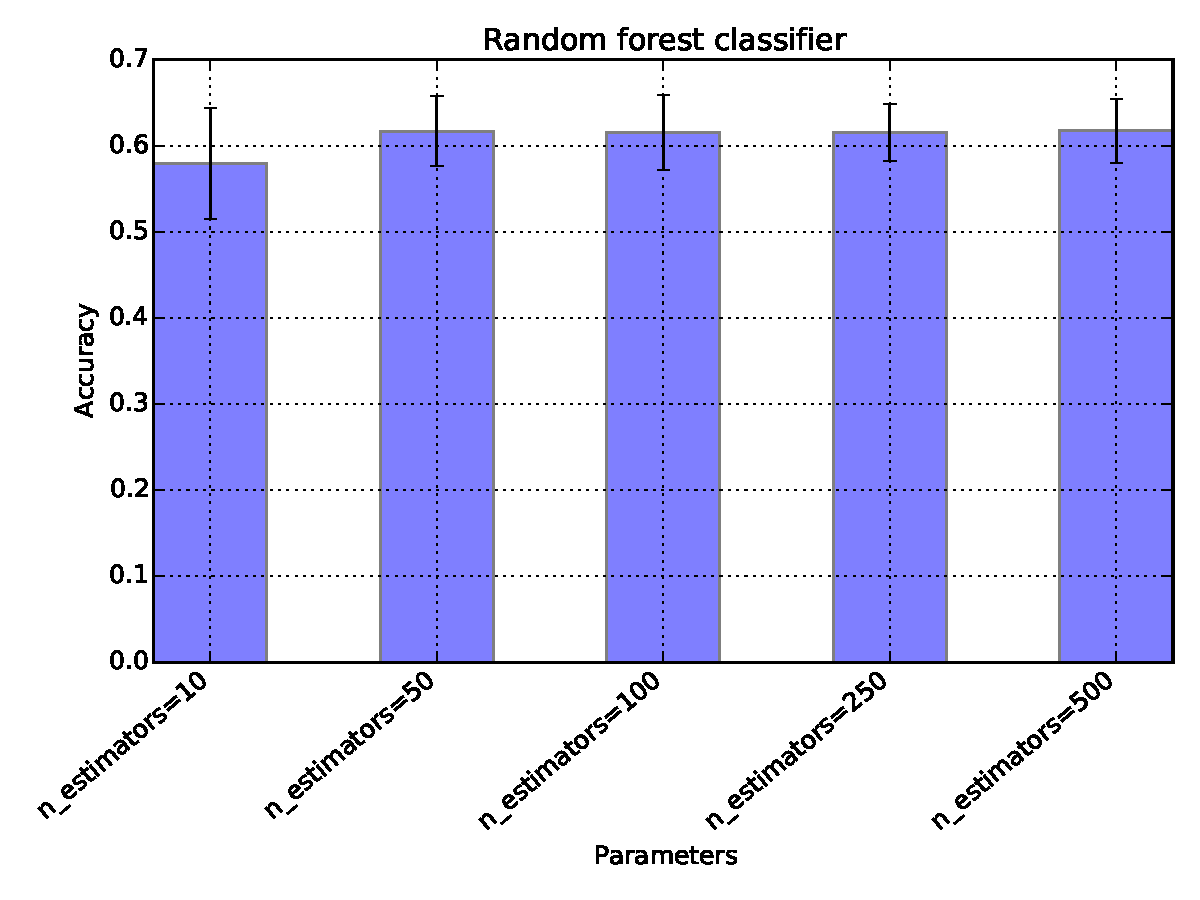
\includegraphics[width=\textwidth]{../plots/experiment_results-Random_forest_classifier.pdf}
    \end{subfigure}~%
    \begin{subfigure}[b]{0.4\textwidth}
      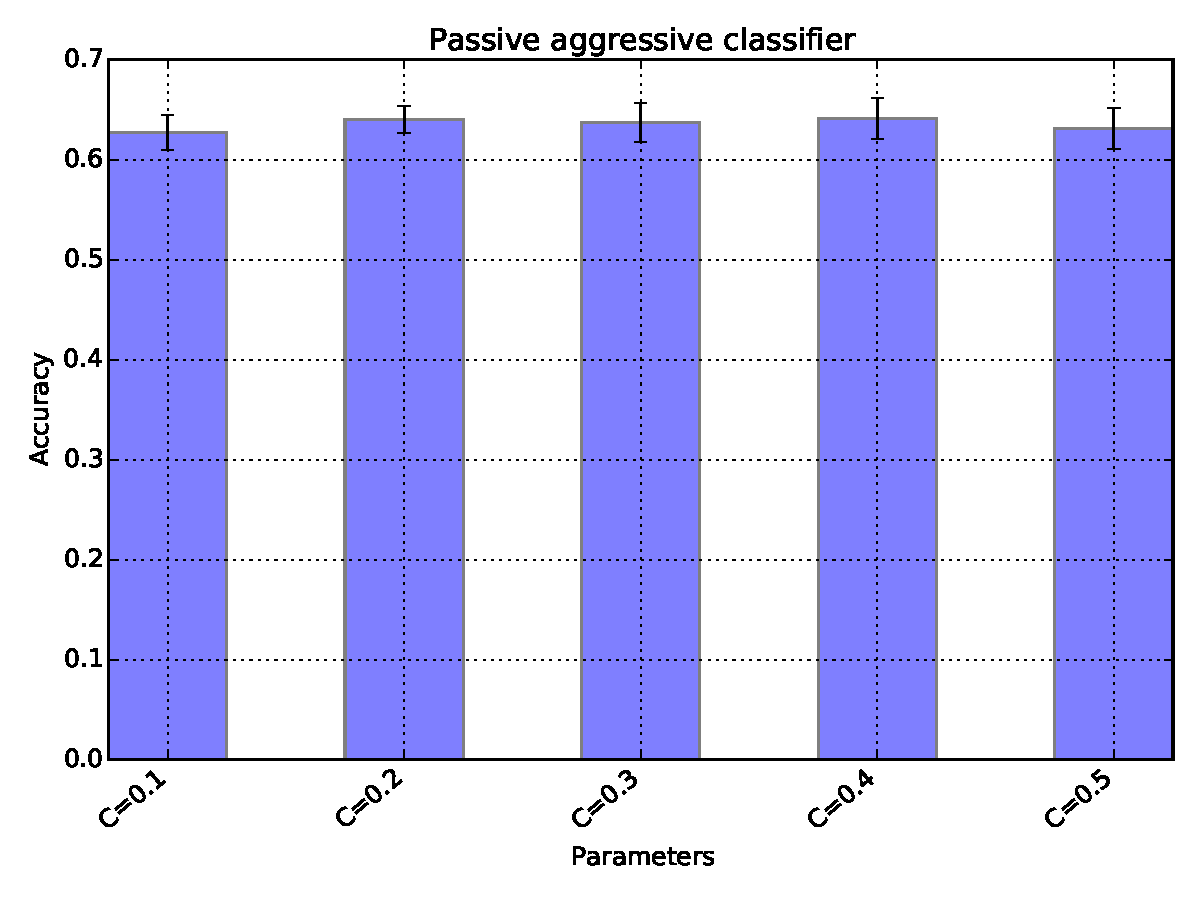
\includegraphics[width=\textwidth]{../plots/experiment_results-Passive_aggressive_classifier.pdf}\\
      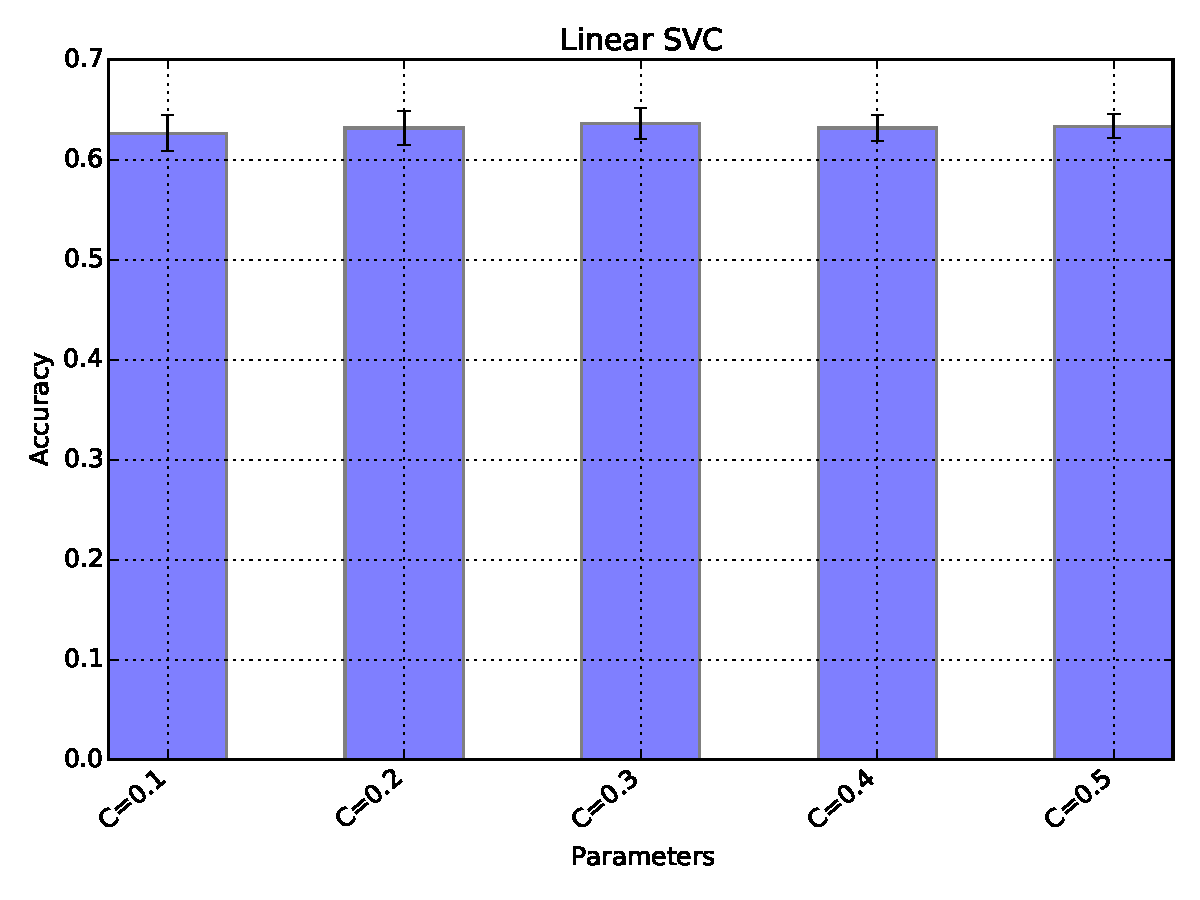
\includegraphics[width=\textwidth]{../plots/experiment_results-Linear_SVC.pdf}
    \end{subfigure}
  \end{figure}
\end{frame}

% Regular slide
\setbeamertemplate{navigation symbols}{}
\begin{frame}[fragile]{Experiments and results (continued)}
\begin{itemize}
  \item Combine all developments to show potential of approach
  \item Sentiment analysis on all commit comments dumps
  \item Goal: visualize languages by negative/positive comments
  \item Bot outputs taken into account: passing tests can be seen as positive, 
    failing tests as negative
  \item Objective comments mostly ignored
\end{itemize}
\end{frame}

% Regular slide
\setbeamertemplate{navigation symbols}{}
\begin{frame}[fragile]{Experiments and results (continued)}
  \begin{figure}
    \centering
    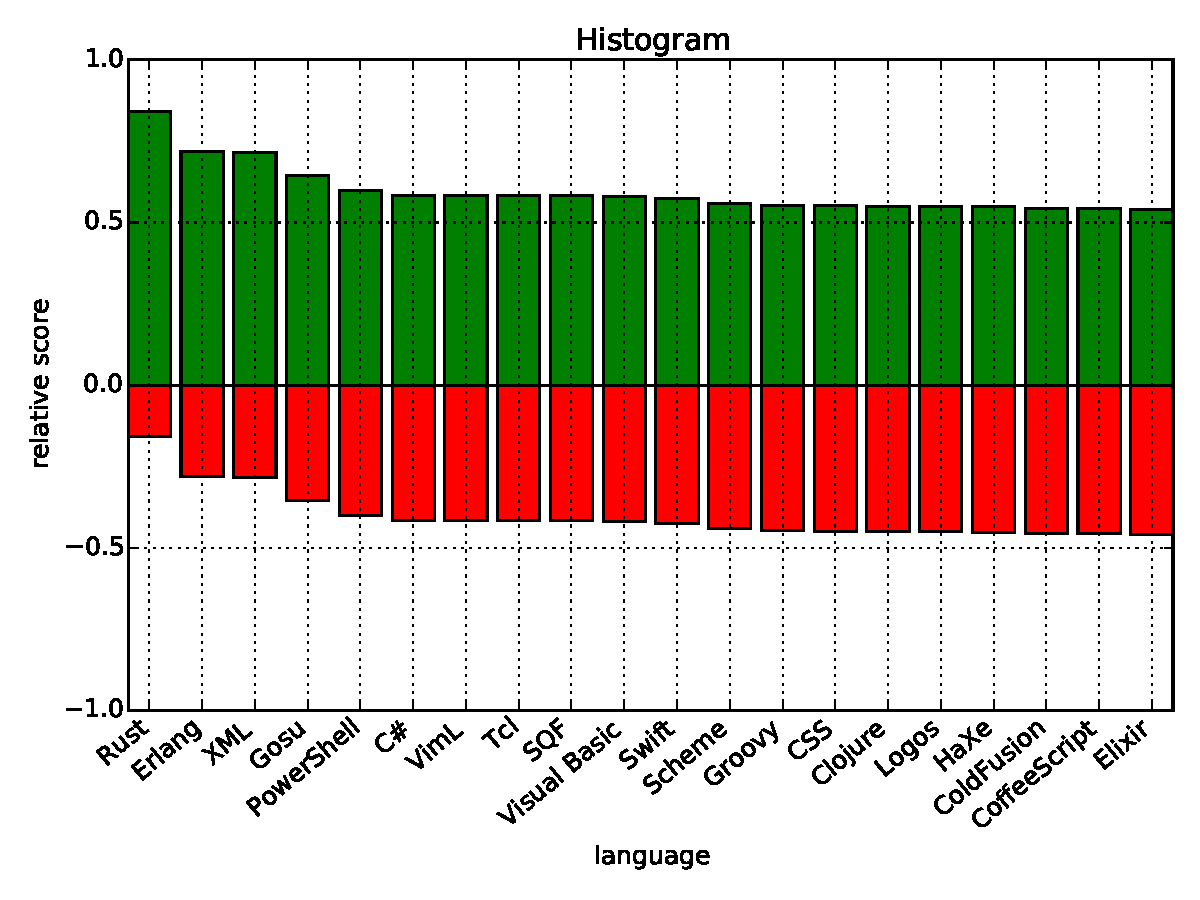
\includegraphics[width=0.7\textwidth]{../plots/all-language-PassiveAggressive-pos.pdf}
  \end{figure}
\end{frame}

% Regular slide
\setbeamertemplate{navigation symbols}{}
\begin{frame}[fragile]{Experiments and results (continued)}
  \begin{figure}
    \centering
    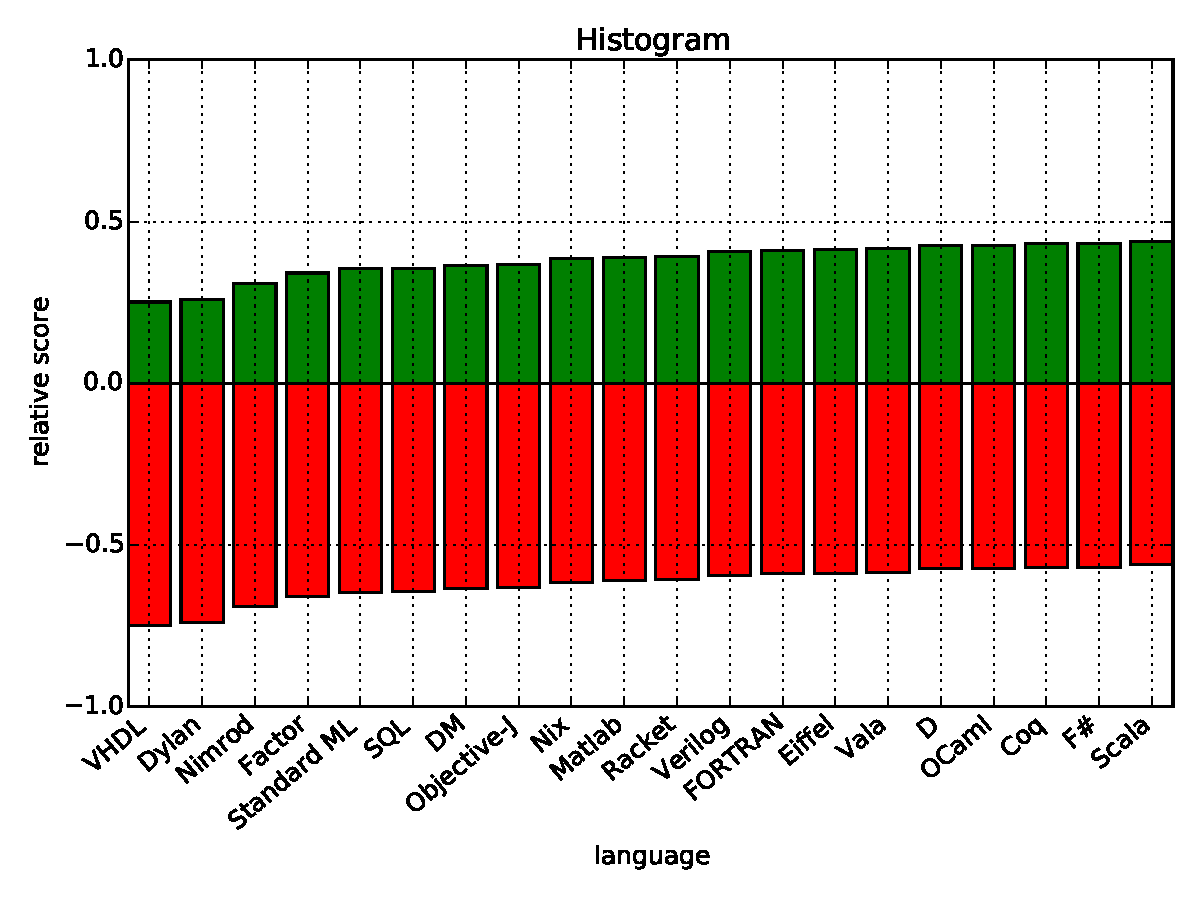
\includegraphics[width=0.7\textwidth]{../plots/all-language-PassiveAggressive-neg.pdf}
  \end{figure}
\end{frame}

% Regular slide
\setbeamertemplate{navigation symbols}{}
\begin{frame}[fragile]{Conclusion}
\begin{itemize}
  \item Implemented a framework for distributed sentiment analysis on GitHub 
    commit comments
  \item Small labeled data set already gives fairly consistent classifiers 
    compared to naive word lists approach
  \item Applied obtained knowledge to visualize most positive and negative 
    languages based on commit comments
  \item Greater potential: can be extended to users, repositories, communities, 
    specific discussions, \ldots
  \item Interesting field of research, especially in combination with 
    distributed data mining
\end{itemize}
\end{frame}

\end{document}
